\documentclass[sw]{iosart2x}
\usepackage[utf8]{inputenc}
\usepackage{graphicx}
% \usepackage{makeidx}
\usepackage[utf8]{inputenc}
\usepackage{mathtools}
\usepackage{breqn}
\usepackage{graphicx}
\usepackage{wrapfig}
\usepackage{lscape}
\usepackage{rotating}
\usepackage{epstopdf}
\usepackage{array}
% \usepackage{minted}
\usepackage{listings}
\usepackage{xspace}
\usepackage{soul}
\usepackage{amsmath}
\usepackage[inline]{enumitem}
\usepackage{csvsimple}

\usepackage[export]{adjustbox}
\usepackage{tabularx}

%%%%%%%%%%% Put your definitions here
\newcommand{\CONSIDER}[1]{{\color{blue}{\textbf{CONSIDER: {#1}}\xspace}}}
\newcommand{\COMMENT}[1]{\hl{ \textnormal{#1}}}
\newcommand{\COMMENT}[2]{\hl{ \textnormal{#1} \textbf{comment:} \textit{#2}}\xspace}
\newcommand{\CHECK}[1]{{\color{yellow}{\textbf{CONSIDER: {#1}}\xspace}}}
\newcommand{\TODO}[1]{{\color{red}{\textbf{TODO: {#1}}\xspace}}}

% abbreviations
\newcommand{\sabio}[0]{SABiO}

% formal definitions
\newcommand{\term}[1]{\textnormal{\textsf{#1}}}
% typed term
\newcommand{\tterm}[2]{{\term{#1}{:}#2}}

% formal matter
\newtheorem{mydef}{Definition}
\newtheorem{myexample}{Example}
%%%%%%%%%%% End of definitions

\pubyear{0000}
\volume{0}
\firstpage{1}
\lastpage{1}


\begin{document}
\def\theequation{A\arabic{equation}}
\begin{frontmatter}
\title{Ontological Foundation of Hazards and Risks in STAMP}
\author[A]{\inits{Ing.}\fnms{Jana} \snm{Ahmad}\ead[label=e1]{jana.ahmad@fel.cvut.cz}%
\thanks{Corresponding author. \printead{e1}.}},
\author[A]{\inits{Ing.}\fnms{Bogdan} \snm{Kostov}\ead[label=e2]{bogdan.kostov@fel.cvut.cz}}
and
\author[B]{\inits{Phd.}\fnms{Andrej} \snm{Lali\v{s}}\ead[label=e3]{lalisand@fd.cvut.cz}}
\runningauthor{N. Surname1 et al.}
\address[A]{Department of Cybernetics, \orgname{Faculty of Electrical Engineering, Czech Technical University in Prague}, \cny{Czech Republic}\printead[presep={\\}]{e1,e2}}
\address[B]{Department of Air Transport, \orgname{Faculty of Transportation Sciences, Czech Technical University in Prague}, \cny{Czech Republic}\printead[presep={\\}]{e3}}

\begin{abstract}
In recent years, there is a growing interest in building safer systems that work in better ways than traditional safety systems. Regarding the daily changes in our community, technology and environment, the causes of accidents and the factors that contribute to these accidents are growing fast with the rapid pace of technological innovation. In fact, we are still searching for the most adequate concepts that would explain and predict safety, what is demonstrated by continuous progress in academia and industry research. In this paper, we contribute to the state-of-the-art by discussing the ontological foundations of hazards and risks. We consider their occurrences in safety systems, specifically in the domain of aviation safety, according to the new accident model STAMP. As a result, we propose a STAMP hazard risk ontology that could help in analyzing accidents and modeling control loop failures according to the theory of STAMP. 
% establishing a common conceptualization regarding aviation safety domain in the new accident model (STAMP: System-Theoretic Accident Model and Processes)
\end{abstract}

\begin{keyword}
\kwd{Aviation}
\kwd{Ontology}
\kwd{Safety}
\kwd{STAMP}
\end{keyword}

\end{frontmatter}

\section{Introduction}
\label{sec:intro}
% TODO - just a test
% context, the progress of safety models, current paradigm in safety (systemic causation models)
With the advent of modern civilization there is a growing interest in building safer systems. High risk industries and sciences are pushing the boundaries of how to view safety and how to improve upon exiting solutions. Different safety models and safety analysis methods were proposed trough out the years~\cite{ECTL2009}. In this regard, we live an era of systemic causation models of safety that attempt to explain causality considering system level and not just its component failures, including phenomena such as emergence, complexity and component interaction accidents. This is especially important as safety has to be addressed typically in socio-technical systems, where the interplay of humans, machines and software matters~\cite{dekker2017}.

% current safety models
The two most recent systemic causation models of safety are STAMP (System-Theoretic Accident Model and Processes)~\cite{leveson2012engineering} and FRAM (Functional Resonance Analysis Method)~\cite{hollnagel2012fram}. Both model systems as compositions of components. STAMP models components as feedback control loops which allow describing objects in three main categories, namely controllers, sensors and actuators (key parts of a feedback control loop). On the other hand, FRAM models components as functions avoiding descriptions of objects by design. 

% state of adoption of the safety models STAMP and FRAM
Both STAMP and FRAM are still being validated by other research \cite{yaosong2012, Pereira2015, Underwood2016, Allison2017, Zhou2018, Patriarca2017add, FUKUDA2016,Patriarca2018}.
%\TODO{add citation for STAMP}. - Resolved AL
These efforts are typically oriented to ad-hoc analyses in practice. Also, there have been proposed some software prototypes supporting modeling with STAMP~\cite{Abdulkhaleq2014a, Abdulkhaleq2015, Abdulkhaleq2016} and FRAM~\cite{Rees2016}. 

% problems of modern safety models
% \TODO{split next sentence into two or more. Add citations FRAM (currently only STAMP)} - Resloved AL
Even though both theories are intelligible and clear when used in simple applications, this ceases to be true for real-industry applications. The analysis can get overly complex and the methodologies associated with STAMP and FRAM would require extensive data~\cite{Kim2016} so as some level of own interpretation and expertise~\cite{Hollnagel2008}. In those cases, it is necessary to bridge the gap between theory and application~\cite{Underwood2016}. 

One of the key obstacles of adopting these models in the industry is the lack of their formalization. Using the same term for different concepts so as different terms for the same concept are some manifestations of this limitation. This paper is part of a collection of work on the formalization of modern theory of safety where we address the issues by ontological analysis and formalization. 

In this paper we focus on the theory of STAMP in the context of hazards and risks. This includes the STPA~\cite{leveson2012engineering} (System-Theoretic Process Analysis) methodology based on the STAMP model, that is intended for the use case of hazards analysis. 

Our contribution includes two ontology modules: the STAMP Hazard and Risk Ontology (SHRO) presented in Section~\ref{sec:shro} and the STAMP Control Loop Hazard Profile (SCLHP) presented in Section~\ref{sec:sclhp}. SHRO describes the concepts Hazard and Risk as understood in traditional safety as well as in STAMP and it is aligned with a novel reference ontology - the Common Ontology of Value and Risk~\cite{unknown}. The SCLHP formalizes the common hazards associated with control loops proposed by the STAMP model. Additionally we validate the Common Ontology of Value and Risk with industry use-cases. We adopt the \sabio{} methodology (Systematic Approach for Building Ontology) \cite{DeAlmeidaFalbo2014} to develop the proposed ontology modules. 

To validate our approach and results, we take the perspective of the aviation industry and its safety management. This work has been done in cooperation with Prague Airport and Czech Airlines Technics who trialled STAMP and STPA in their operations within a research project. This is an important part since industry perspective can directly assess the usability and applicability of the proposed solutions. Industry experts also directly participated in the research activities.

The remainder of this papers is organized as follows: In Section~\ref{sec:back}, we detail STAMP, UFO and Risk Ontology used to provide the ontological foundations for our work. Section 3 shows the developed STAMP Hazard and Risk Ontology (SHRO), which is analyzed in Section 4. Section 5 shows ontology validation and section 6 adds more details on the related work. Section 7 concludes the paper.

% From the conceptual model perspective, we are not the first to analyze factor and risk. For example, the authors in [The Common Ontology of Value and Risk] formally characterize the process of ascribing risk as a particular case of the process of ascribing value. Goal-Risk framework [2], an approach designed to
% support risk analysis in the context of requirements engineering. Archimate [6], in which risks are analyzed in the context of enterprise architecture models. And in [] an Ontology to define Ramp Error Decision Aid (REDA) Contributing Factors.




% \subsection{Contributions}
%TODO rewrite according to the actual contributions
% In this work we contribute with:
% \begin{enumerate}
    % \item Alignment of the concepts of Risk and Hazard as used in STAMP with the Risk Value ontology.
    % \item Modeling control loop failures selected by the STAMP methodology % according to the hazard and risk ontology based on the Risk Value % ontology.
    % \item Proposing a STAMP hazard risk ontology and how it could help for establishing STAMP methodology to industry
% \end{enumerate} 


\section{Background}
\label{sec:back}
This section provides fundamentals for our research. It deals both with safety and ontology engineering, provides definition of key concepts and industry example. 

\subsection{STAMP: Hazards and Risks}
\label{sec:back:stamp}
\TODO{BK: Write how STAMP context for Hazard and Risk.}

These two concepts serve successfully for a couple of decades (since the invention of HAZOP methodology~\cite{kletz2001hazop}) the very core of industrial safety management and are often part of industry standards (e.g. in aviation see~\cite{ICAO2018}). The STPA methodology using the STAMP model builds upon the cornerstones of HAZOP and provides for some additional steps and guidance, in line with the perspective of feedback control theory~\cite{doyle2009feedback}. However, the above-mentioned shortcomings of STAMP hold for STPA as well, and current safety management using hazards and risks as in HAZOP has its clear limitations, most of the apparent being the inability to progress any further on the safety of current operations~\cite{dekker2017}.

As already mentioned, STAMP is a safety causation model that sees problem of safety as a feedback control problem. With respect to this, the theory of STAMP proposes generic control loop issues that can be mapped to specific system (particular network of control loops) and used to derive hazards or support accident/incident investigation. The generic control loop with classification of control problems is depicted in Fig.~\ref{fig:loop}. 

The theory is not completely new but builds upon the heritage of Rasmussen~\cite{Rasmussen1997}, Perrow~\cite{Perrow1999} and other successful practices in safety (as the already mentioned HAZOP). This is clear from how the theory of STAMP defines hazard~\cite{leveson2012engineering}:
\begin{mydef}
\label{def:hazard}
A system state or set of conditions that, together with a particular set of worst-case environmental conditions, will lead to an accident (loss).
\end{mydef}
As an example, the adopted definition of hazard in civil aviation (by International Civil Aviation Organization) is "\emph{A condition or an object with the potential to cause or contribute to an aircraft incident or accident.}"~\cite{ICAO2018} The theory of STAMP updates conventional definitions of hazard to include the system perspective (system state), but does not reinvent the concept. Similar situation regards risk, which is defined by STAMP~\cite{leveson2012engineering} as:
\begin{mydef}
\label{def:risk}
A function of the hazard level combined with (1) the likelihood of the hazard leading to an accident and (2) hazard exposure or duration.
\end{mydef} 
This definition conforms to what is usually regarded as risk in different industries and does not introduce new notions (concepts). 

To demonstrate the meaning of the concepts \emph{hazard} and \emph{risk} and their relation, consider the following example: 

\begin{myexample}
\label{ex:birdstrike}
A bird strike is a type of incident in which a bird collides with an aircraft. 
Let's consider a specific bird strike incident. The cause/factor of that incident is the presence of a flying bird during landing of an airplane. The damage of the aircraft requires minor repair of the airplane fuselage.
\end{myexample}

Based on example~\ref{ex:birdstrike}, we can say that birds flying near a runway during landing/takeoff of an aircraft is a hazardous situation. This hazardous event increases the risk (probability) of the occurrence of a bird strike event. Note that both hazard and risk are not associated with a specific event. They represent empirical knowledge used to predict the probability and the level of loss given a specific situation arises. Finally, this knowledge is always extracted from concrete events (e.g. investigation of an incident analysis of a hypothetical incident). Risk is based on the loss (the incident itself) while hazards are based on factors of incidents.


STAMP theory supports multiple use cases (designing a system, operations, investigation and similar), each with some specific perspectives, but we will not focus on these as they fall outside the scope of this paper.

\begin{figure*}
\begin{center}
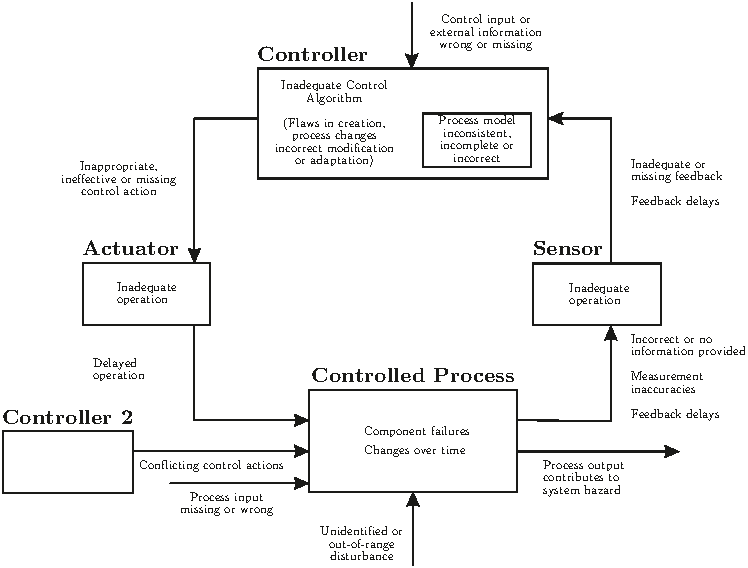
\includegraphics[width=0.7\textwidth]{images/Fig_Loop.pdf}
\end{center}
\caption{Generic control loop with issues classification as per STAMP (adopted from~\cite{leveson2012engineering})}
\label{fig:loop}
\end{figure*}


\subsection{Industry example}\label{sec:example}
Due to confidentiality restrictions, this sections does not provide industry example from the environment of Prague airport or Czech Airlines Technics, where this project was carried out. We decide to exemplify our approach using industry example provided directly by the author of STAMP~\cite{leveson2012engineering}, from the domain of military aviation, namely the friendly fire accident from April 15, 1994 that occurred in Iraq. On that day, two U.S. Air Force interceptors patrolled an area and mistakenly shot down two U.S. Army helicopters carrying 26 people, who all died in the accident. 

Detailed investigation using STAMP principles is demonstrated directly by the author of STAMP. For the sake of practicality we take only the last three minutes of the accident, as follows:
\begin{itemize}
  \item Time 0728: Lead interceptor pilot has visual contact with unidentified helicopter at 5 nautical miles.
  \item Time 0728: Lead interceptor pilot conducts identification pass and asks his wingman, using phraseology, whether he sees two enemy (Iraqi) helicopters.
  \item Time 0728: Wingman interceptor pilot confirms seeing two helicopters.
  \item Time 0729: Lead interceptor pilot instructs his wingman to disarm missiles, reports to the controllers of the operation (supervising flights in the area) that he engaged some targets.
  \item Time 0730: Interceptors fire at helicopters, they are hit by missiles.
\end{itemize}

The safety control structure involved in the last minutes is depicted in Fig.~\ref{fig:example}. Each of the figure elements consists of a separate control loop, where the simplified control structure above the pilots involves complex network of various control loops. Considering the definition of hazard from previous section, the system states and conditions can be derived from all involved control loops in the control structure so as from the relations between them. With regard to the last minutes of the accident mentioned above, example of hazard is early control action of the lead interceptor pilot who, being apparently in a rush, did not check thoroughly that his wingman in time 0728 actually did not confirm seeing two enemy helicopters but only two helicopters. Note that in Fig.~\ref{fig:example}, control-feedback relations are only hierarchical; there is only indirect coordination between the interceptors and the helicopters for which the mission control is responsible.

\begin{figure}[b]
\begin{center}
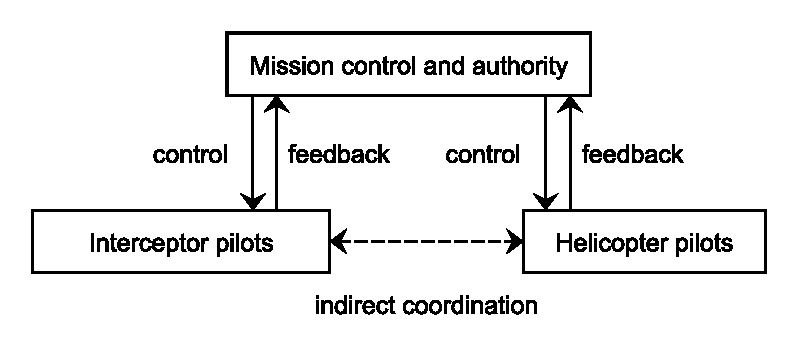
\includegraphics[width=0.5\textwidth]{images/Fig_Example.pdf}
\end{center}
\caption{Control of interceptors (fighters) and helicopters in the example mission (adopted from~\cite{leveson2012engineering})}
\label{fig:example}
\end{figure}


\subsection{STAMP Ontology}
As already indicated, this paper deals only with the ontological foundations of hazards and risks, but the work is part of research project which aims to formalize the entire theory of STAMP. The entire ontology modularization is depicted in Fig.~\ref{fig:modules}. This section deals only with the modules "Hazards and Risks" and "Control Loop Hazards".

\begin{figure}
\begin{center}
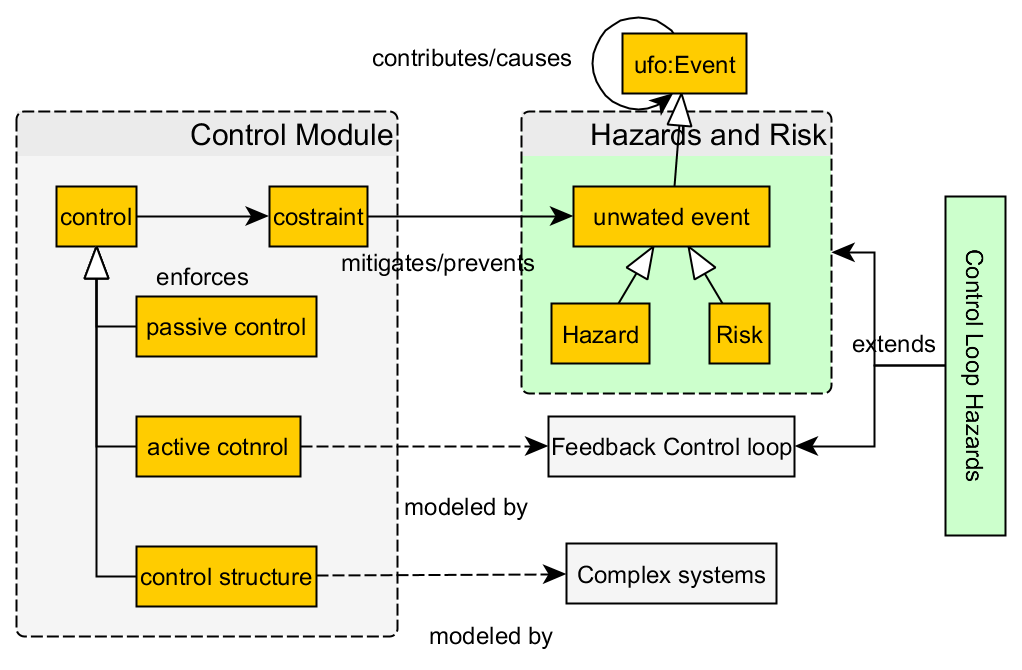
\includegraphics[width=0.5\textwidth]{images/modules.png}
\end{center}
\caption{STAMP modules}
\label{fig:modules}
\end{figure}


\subsection{Ontology and Ontology Engineering Methodology}
\label{sec:method}
The term ontology (in other words the study of existence) originates in philosophy. In computer science, there are several definitions of what is an ontology. We adopt the definition found in \cite{Studer1998} -- "\emph{An ontology is a formal, explicit specification of a shared conceptualization}". 

Engineering an ontology is a complex process. There are many methodologies found in the literature, e.g., agile methodology, RapidOWL \cite{Auer2006} and Methontology \cite{Fernandez-Lopez1997}. In this work, we are using a more recent methodology called \sabio{} (Systematic Approach for Building Ontologies). This methodology proposes five consecutive steps: \begin{enumerate*}
    \item Purpose Identification and Requirements Elicitation; 
    \item Ontology Capture and Formalization; 
    \item Design; 
    \item Implementation and 
    \item Testing 
\end{enumerate*}. The first two steps build the so called \emph{domain-reference} ontology which captures key knowledge of the domain. The next two steps focus on the design and implementation of a \emph{domain-operational} ontology into a formal machine-readable representation of the domain-reference ontology developed in the first two steps. The domain-operational ontology is designed to be used in software solutions. Finally, the last step evaluates the ontology w.r.t. to functional requirements defined in the first step or throughout the engineering process. 

Furthermore, \sabio{} specifies five support activities which are parallel to the process described above. A short description of the most relevant support activities is shown below:
\begin{itemize}
\item Knowledge Acquisition - interviews with domain experts, literature analysis
\item Reuse - reuse of existing ontologies/conceptualizations
\item Documentation - document the engineering process
\item Evaluation - evaluation of intermediary artifacts
\end{itemize}
More information about \sabio{} methodology can be found at \cite{DeAlmeidaFalbo2014}.
% Describe specific activities
% - foundational ontology patterns

The engineering efforts were achieved by a team consisting of two ontology engineers, two domain experts and two potential ontology users. The ontology engineers and the domain experts have experience \cite{Kremen2017a,Kostov2017b} with building ontologies grounded in the Unified Foundational Ontology (UFO). Both ontology users represent safety management departments of the two commercial partners participating in the research, i.e. Prague Airport and Czech Airline Technics. 

Section~\ref{sec:back:onto:risk} describes a common reference ontology of Risk and Value which is grounded in UFO. \COMMENT{ JA: (I couldn't understand this sentence:)This ontology is used for the 
Following this section}, the paper is structured along the five main activities in the \sabio{}.

\subsection{Ontological Foundations}
\label{sec:back:onto}
This section details the ontology engineering used in this work, i.e. the reuse of the Common Ontology of Value and Risk, so as the UFO ontology.

\subsubsection{The Common Ontology of Value and Risk}
\label{sec:back:onto:risk}
In the Common Ontology of Value and Risk \cite{unknown} grounded with UFO, the authors have presented an ontological analysis of risk which clarifies the connections between the concepts of value and risk. The ontology discusses three different perspectives of risk: (i) the relational perspective that describes risk as the relationship of ascribing risk, which the authors classified as Risk Assessment; (ii) the experiential perspective that considers risk as a chain of events that impacts on an agent’s goals or intentions, which the authors labelled as Risk Experience; (iii) and the quantitative perspective that describes risk as a quantitative notion which they labelled as Risk, i.e., it describes the risk by means of the Risk qualities inhering in particular relations. 
% \COMMENT{ AL: This sentence does not make sense to me, more over, I think no sentence should start with "I.e." or "E.g.", nor should it miss the subject}

Furthermore, because the ontology aims to discuss the connections between risk and value, the authors presented an ontological analysis of using value by (i) discussing the impact of likelihood of events on value, (ii) describing value as experience, its structure and the objects that participate in this experience, and (iii) clarifying the role of dispositions in value creation.

From the previous different perspectives on risk and value, the authors propose the Common Ontology of Value and Risk, formalized in OntoUML \cite{Guizzardi2005c}.

\paragraph{Relation to our approach.}
The current version of the Common Ontology of Value and Risk, however, does not completely describe the domain of risk management as it lacks safety-related concepts such as mitigation and control strategies. In our paper, based on this ontology and with respect to the principles of Unified Foundational Ontology, we present STAMP hazard and risk ontology which analyzes risks and hazardous states contributing to loss events in safety domain in accordance with STAMP. 

\subsubsection{Unified Foundational Ontology (UFO)}
\label{sec:back:onto:ufo}
% Ontologies are used to specify the meaning of terms of some domain, categorizing it and setting relationships among these terms. They define basic concepts like objects, relations, events, processes, situations, and other high-level domain-independent categories. A \emph{top-level ontology} is an ontology that describes general concepts that are common to multiple domains. There are many well-known foundational ontologies, like (DOLCE)\cite{Mylopoulos1992}, Unified Foundation Ontology (UFO) \cite{Guizzardi2005b}, and Basic Formal Ontology (BFO) \cite{Grenon2004}.

% For the purpose of this study, we have chosen to build our proposal on top of UFO. Because of (i) our experience in using UFO in various conceptual model-based domains ~\cite{Kostov2017b}, (ii) UFO addresses many essential aspects for conceptual modeling, which have not
% received a sufficiently detailed attention in other foundational ontologies \cite{Guizzardi2005b}, (iii) the availability of its formal translation to OWL~\cite{DBLP:conf/jowo/BenevidesBGP17}, (iv) availability of OntoUML, an ontology modeling language based on UFO \cite{Guizzardi2005b}. 

UFO is a top-level foundational ontology that has been developed based on a number of theories from Formal Ontology, Philosophical Logic, Philosophy of Language, Linguistics and Cognitive Psychology \cite{Guizzardi2005c}. Its main concepts fundamental for this work are sketched in the UML class diagram
% \footnote{The figure is a straightforward visualization of a fragment of UFO axiomatization in OWL, e.g. $\term{Trope} \sqsubseteq \forall \term{inheresIn} \cdot \term{Individual} \sqcap \exists \term{inheresIn} \cdot \term{Individual}$ denotes the edge from $\term{Trope}$ to $\term{Individual}$. See \cite{DBLP:conf/jowo/BenevidesBGP17} for details.}
in Figure~\ref{fig:fu}. UFO describes endurants that are static objects (UFO-A)\cite{Guizzardi2005b}, perdurants or events (UFO-B)~\cite{Guizzardi2013} and social agents (UFO-C) built on top of UFO-A and UFO-B \cite{Guizzardi2010a}. UFO splits entities into endurants and perdurants which are Individuals, entities that exist in reality and possess an
identity that is unique (\term{Endurant} $ \sqsubseteq $ \term{Individual}) (\term{Perdurant} $ \sqsubseteq $ \term{Individual})\footnote{We reuse Description Logic formalization of basic UFO concepts introduced in ~\cite{DBLP:conf/jowo/BenevidesBGP17}}. Endurants can be observed as complete concepts in a given time snapshot and they can be any object (e.g. an agent, aircraft)  (\term{Object} $ \sqsubseteq $  \term{Endurant}), or its tropes (e.g. speed, location) (\term{Trope} $ \sqsubseteq $  \term{Endurant}), that exist as long as an object they inhere in exists (\term{Trope} $ \sqsubseteq $  ($ = $ 1 \term{inheresIn}$\cdot$\term{Object})). 

% \CONSIDER{interval}
Perdurants only partially exist in a given time snapshot. They involve events (\term{Event} $ \sqsubseteq $  \term{Perdurant}), situations (\term{Situation} $ \sqsubseteq $  \term{Perdurant}) and object snapshots (\term{ObjectSnapshot} $ \sqsubseteq $  \term{Perdurant}). 

Events can be either atomic or complex (\term{Event} $ \sqsubseteq $  (\term{AtomicEvent} $ \sqcup $ \term{ComplexEvent})), they occur in time and have participants ( \term{Event} $ \sqsubseteq $ ($\ge$ 1  \term{hasParticipant} $\cdot$ \term{Object})) and complex events have parts ($\exists$ \term{hasEventPart} $\cdot$ $\top$ $\sqsubseteq$ \term{ComplexEvent}) \cite{Guizzardi2013}. An event occurs in a certain \term {situation} at a certain point in time, and transforms it to another situation. ObjectSnapshot: is an immutable state description of an object within a situation. Situation: is a snapshot of object states valid in the given temporal range.

Moreover, UFO defines Dispositions which are Intrinsic Moments (\term{IntrinsicMoments} $ \sqsubseteq $  \term{Trope}), i.e., existentially dependent entities that are realizable through
the occurrence of an Event  (\term{Dispositions} $ \sqsubseteq $  \term{Trope}). This occurrence brings about a Situation \cite{Guizzardi2014}. In other words, UFO considers dispositions as properties that are only manifested in particular situations or the occurrence of certain triggering events, and that can also fail to be manifested (\term{Event} $ \sqsubseteq $  ($ = $ 1 \term{isManifestedBy}$\cdot$\term{Dispositions})). Dispositions inhere in particular objects (\term{Dispositions} $ \sqsubseteq $  ($ = $ 1 \term{inheresIn}$\cdot$\term{Object})). For example, security flaw in an information system is manifested by event of stealing sensitive data that brings about non safe situation.

Additionally, UFO introduces the notion of agents (\term{Agent} $ \sqsubseteq $  \term{Object}), i.e., proactive objects with an intention (e.g. a person, or an animal), their intentions, commitments and actions they perform ($\exists$ \term{performs} $\cdot$ $\top$ $\sqsubseteq$ \term{Object}) \cite{Guizzardi:2004:TOF:2156041.2156051}, services \cite{unknown1}, and power type, i.e., universal types 
whose instances are individuals in the subject domain \cite{CARVALHO20173, gagc2015toap}.


\begin{figure*}
\begin{center}
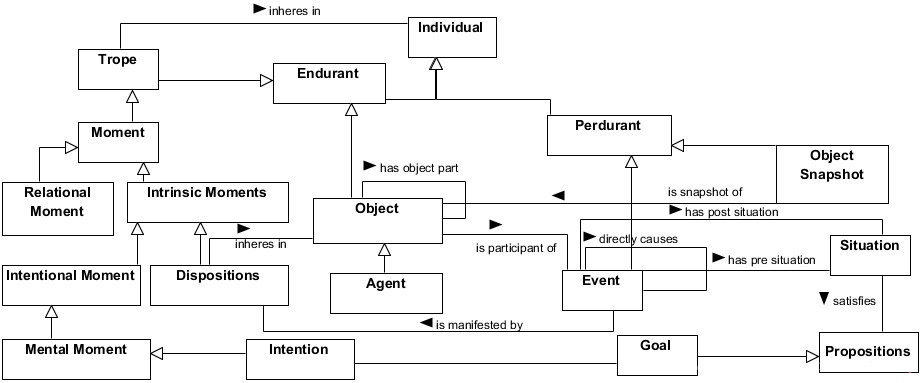
\includegraphics[width=\textwidth]{ufod}
\end{center}
\caption{Main concepts of UFO}
\label{fig:fu}
\end{figure*}

We selected UFO for this work because of (i) our experience with using UFO in various conceptual model-based domains ~\cite{Kostov2017b,Kremen2017a}, (ii) UFO addressing many essential aspects for conceptual modeling, which have not
received sufficiently detailed attention in other foundational ontologies \cite{Guizzardi2005b}, (iii) the availability of its formal translation to OWL~\cite{W3COWLWorkingGroup2012}, (iv) the availability of OntoUML, an ontology modeling language based on UFO \cite{Guizzardi2005b}.


\section{Ontology Purpose Identification}
\label{sec:purpose}
The purpose of the ontology is identified with help of the oenology users and safety domain experts and it is based on the knowledge acquisition activity dopcumented in Section~\ref{sec:back:stamp}   in safety The purpose of the ontology is to be able to represent hazard and risk knowledge about the industry example presented in Section~\ref{sec:example} \COMMENT{JA: not only represent the example, but we aim to represent all hazards and risk in the domain, it would be very week to say represent one example}. With the help of experts and ontology users, we identify key terms in the example and the STAMP literature. The fragment of the STAMP terminology dealing with hazards and risks can be divided into two modules, the STAMP Hazard and Risk Ontology (SHRO) and the STAMP Control Loop Hazard Profile (SCLHP). The terms related to the SHRO ontology are shown in Table~\ref{tab:purpose} 
and for SCLHP are the shown in Fig.~\ref{fig:loop}.

\begin{table}\label{tab:purpose}\caption{Concepts and relations capturing the purpose of the SHRO ontology.}
% \csvautotabular{tables/stamp-hr-terms.csv}
%\csvautotabular{tables/stamp-risk-alignment.csv}
\csvautotabular{tables/shr-terms.csv}
\end{table}

Based on this terminology, we define with help of experts and ontology engineers the following competency questions which serve to verify the ontology. SHRO aims to answer the following competency questions (CQs), which were derived from related STAMP literature~\cite{leveson2012engineering, Leveson2004} or from domain experts:  
% \CONSIDER{Revize competency questions. First, start with questions about entities Hazard, Risk, . For example (CQ5, CQ5a, CQ5b). Second, continue with the relations between the entities. Third, the questions should be organized two categories, where the first category may be questions about specific events (e.g. accidents/incidents and their factors) and the second questions about future events (or event types) (hazards and risks)}
\begin{itemize}
\item \emph{CQ1:} What is the accident/What Happened?
   \item \emph{CQ2:} What are the hazards in the controlled system?
    % \item \emph{CQ5a:} \CONSIDER{What are the Risks of the system?}
    % \item \emph{CQ5b:} \CONSIDER{What are the type of Accidents of the system?}
    \item \emph{CQ3:} How does risk accumulate concerning specific hazard?
    % {I like this question but I think that it should be written in another way or may be an example can clarify the point.}
    %   What is the risk that resulted from a specific hazard?
    \item \emph{CQ4:}
    What are the factors of a given Accident
    % \COMMENT{Why a specific accident happens?}{I prefer: "What are the factors of a given Accident"}
   
    \item \emph{CQ5:} What is the STAMP failure classification?
    % {Not a clear question.}
    \item \emph{CQ6:} Where is the potential for inadequate control actions (possible control flaws)?
    
   
   
    % \item \emph{CQ9} Which hazards were violated?
      \item \emph{CQ7:} Where can be identified responsibility for specific risks?
    % Who responsible for specific occurrence?
    \item \emph{CQ8:} Which objects participate in a specific occurrence?
    
\end{itemize}


\section{Aligning STAMP Hazard and Risk Concepts to the Common Ontology of Value and Risk}
\label{sec:align-shro}
SRHO describes the concepts Hazard and Risk as understood in traditional safety as well as in STAMP and it is aligned with a novel reference ontology the Common Ontology of Value and Risk~\cite{unknown}. The ontology has been composed from several risk assessment methodologies, used by different industries and domains. The ontology is grounded with the Unified Foundational Ontology (UFO) \cite{Guizzardi2005c} and as such provides for the most recent and complete conceptualization of risk. 
\CONSIDER{This section should explain the key Hazard-Risk related terms used in safety and STAMP.}

\section{STAMP Hazard and Risk Ontology (SHRO)}
\label{sec:shro}

% As mentioned before, we built our STAMP Hazard and Risk Ontology (SHRO) based on the Common Ontology of Value and Risk~\cite{unknown} on top of the Unified Foundational Ontology (UFO) \cite{Guizzardi2005c}. \COMMENT{ AL: To me, the first sentence appears rather repeating, of no new value to the reader here. I propose to delete it.}
We designed SHRO for describing safety issues and increasing the awareness of analytic methods and tools for safety analyses in the domain of aviation, focusing on the STAMP accident model, but the ontology is not limited to aviation industry. Our strategy is to analyze STAMP-based safety events that lead to incidents or accidents and explain STAMP-based hazards or factors, that contribute to safety events. Such approach ensures reusability of the ontology for other high-risk industries. The ontological foundational model of SHRO is presented in Fig.~\ref{fig:f2}. The concepts are assigned colors as follows: \emph{yellow} - concepts native to SHRO; \emph{blue} - concepts reused from the Common Ontology of Value and Risk; \emph{white} - UFO concepts reuse.

\begin{figure*}
\begin{center}
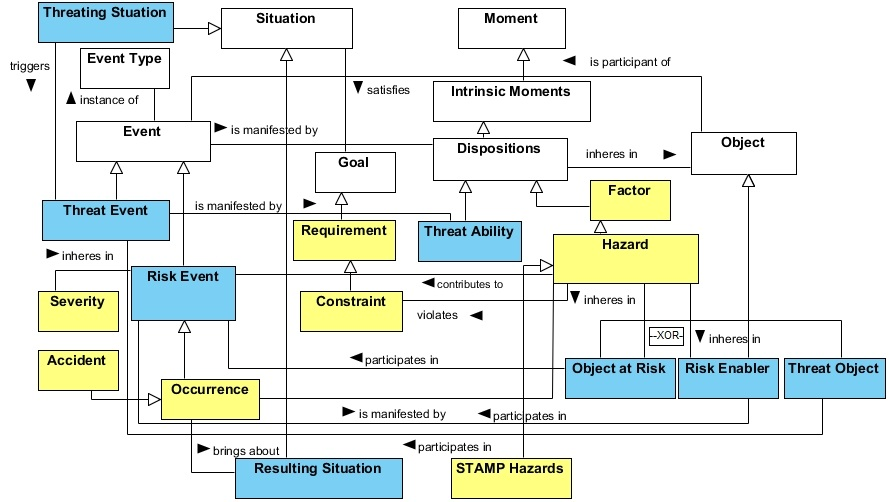
\includegraphics[width=\textwidth]{shro.jpg}
\end{center}
\caption{Main concepts of SHRO grounded in the Common Ontology of Value and Risk and UFO.}

\label{fig:f2}
\end{figure*} 


% \COMMENT{ AL: Please correct typos in Fig. 5: "Severity", "STAMP Hazrds". Do the same for Fig. 4: "Intention" and Fig. 6: "Unsafety Situation" (should be "Unsafe Situation"), "two U.S. Army helicopters shut down" (should be "Two U.S. Army helicopters shot down), "STAMP Hazards", check usage of capitals etc.}

 

% To explain \emph{CQ1} and \emph{CQ2}.
According to definition~\ref{def:hazard} hazard concept describes any factor that causes or contributes to an unplanned and undesired loss event. That loss may involve human death and harm, but it may also include other major occurrences, including system or equipment damage, and information losses. Thus, there are different physical or social objects participating in the occurrence of hazard. In SHRO, we adopt three object roles that participate in a loss, defined in the Common Ontology of Value and Risk: 
\begin{itemize}
    \item Threat Object: a person or any object who poses danger to an asset (via threat event, e.g., attacks), i.e. the objects participating in a threat event. An example of a Threat Object is a hacker of safety information.
    \item Object at Risk: an object, which is exposed to potential damage. Objects at risk are constituted around traits such as loss, vulnerability, and need for protection, e.g., a person in an accident. Therefore, they deserve attention and care. For example, information should be protected from a hacker attack.
    \item Risk Enabler: the main responsible object for risk event or accident. It has inherent hazards in the sense that it refers to something that is identified as dangerous, e.g. the controller in STAMP model.
\end{itemize}
Axiom~\ref{ax:a1} captures this notion in our ontology: if a risk or loss event is manifested by a hazard, then this hazard inheres in an object (Risk Enabler) who participates in this loss event.  
% hazard \emph{\term{h}} inheres in any role of objects, it causes a risk event \emph{\term{re}} or threat event \emph{\term{te}} regarding the object's role.
 
% \begin{equation} \label{eq1}
% \begin{split}
%   \forall\term{to}: ThreatObject, \term{oir}: ObjectinRisk,~ ~\\
%     \term{reo}: RiskEnablerObject, \term{h}: Hazards,\\
%     \term{te}: ThreatEvent, 
%   \term{re}: RiskEvent~ ~ ~ \\
%      \term{inheresIn}(\term{h},\term{to})~ \land~  \term{inheresIn}(\term{h},\term{oar})~ \land 
%   \term{inheresIn}(\term{h},\term{reo}) 
%         \rightarrow~(
% \term{isParticipantOf}(\term{te}, \term{oe})~ \land~ \term{isParticipantOf}(\term{re}, \term{oar}) )
% \end{split}
% \end{equation}

% \COMMENT{see latex source}
% \begin{dmath}
% \forall \term{to},~\term{oar},~\term{reo},~\term{h1, h2, h3},~\term{to},~\term{te},~\term{re}\\
% \term{inheresIn}(\term{h1},\term{to})~ \lor~  \term{inheresIn}(\term{h2},\term{oar})~ \lor ~ \term{inheresIn}(\term{h3},\term{reo}) \\ \rightarrow~(
% \term{isParticipantOf}(\term{oe}, \term{te}) \land \\ \term{isParticipantOf}(\term{re}, \term{oar})), \\
% \tterm{to}{ThreatObject}, \\ \tterm{oar}{ObjectAtRisk}, \\ \tterm{reo}{RiskEnablerObject}, \\  \tterm{h1, h2, h3}{Hazard}, \\ \tterm{te}{ThreatEvent}, \tterm{re}{RiskEvent}
% % \tterm{te}{ThreatEvent}\land  \tterm{re}{RiskEvent}\land \\
% \end{dmath}

\begin{dmath}
\label{ax:a1}
$\forall \term{h},~\term{re}
~ ~ \term{manifestedBy}(\term{re}, \term{h})  \rightarrow~ \exists~\tterm{reo} {RiskEnablerObject}\\  \term{inheresIn}(\term{h}, \term{reo}) \land \\ \term{isParticipantOf}(\term{reo}, \term{re}))$,~ 
 \\ \tterm{h}{Hazard}, \tterm{re}{RiskEvent}
\end{dmath}

% To answer \emph{CQ3} and \emph{CQ4},
% \COMMENT{see latex source}

As in the Common Ontology of Value and Risk, each risk and threat event is manifested by some vulnerabilities, weak points or hazards that cause or lead to these events, i.e. accident's cause can be described, using STAMP, by identifying relevant safety constraints,
%TODO - BK: What if there was no constraint?
that were violated by vulnerabilities or hazards. Example could be two aircraft violating minimum separation requirements  \cite{leveson2012engineering}. However, there are situations in which the there is no violation of a constraint. One example is when an accident, such that the safety control structure does not account for, occurs. Axiom~\ref{ax:topconstraints} ensures that occurrence of any loss event is considered a constraint.
\begin{dmath}
\label{ax:topconstraints}
\forall \tterm{le}{LossEvent} \rightarrow \exists \tterm{c}{AvoidEventConstraint} ~ ~ \term{eventToAvoid}(c,e)
\end{dmath}

According to STAMP theory, a proper analysis and understanding of these hazards can resolve major part of safety issues and significantly reduce risk in everyday operations.
In axiom~\ref{ax:a3}, if any risk event \term{re} happened due to any hazard \term{h}, then this hazard doesn't respect the safety constraints \term{c} but violates them:

% \COMMENT{see latex source}
\begin{dmath}
\label{ax:a3}
$\forall \term{h},~\term{re}
~ ~ \term{manifestedBy}(\term{re}, \term{h})  \rightarrow~ \exists~\tterm{c}{Constraint} \\  \term{violates}(\term{h}, \term{c}) $,~ 
 \\ \tterm{h}{Hazard}, \tterm{re}{RiskEvent}
\end{dmath}

% regarding \emph{CQ5}, and \emph{CQ6}.
Furthermore, losses result from component failures as shown in Fig~\ref{fig:loop}, e.g. disturbances external to the system, interactions
among system components, and behaviour of individual system components. That leads to hazardous system states, which are denoted in Fig.~\ref{fig:f2} as STAMP Hazards (STAMP Failures). Example of hazards includes
% train doors closing while people going inside and 
% the answer of \emph{CQ5}, and \emph{CQ6} 
%TODO - BK: Death of a patient seams as an accident, not a hazard?
medical mistakes which are manifested by death of patients, where the loss event is caused by medical mistake hazard. Consequently, STAMP hazard and risk ontology must obey axiom~\ref{ax:a4} that hazard \term{h} is manifested by risk event \term{re} if and only if this hazard contributes to the risk event.

\begin{dmath}
\label{ax:a4}
$\forall\term{re}, \term{h}  ~  ~ \term{ismanifestedBy}(\term{re},\term{h}) 
~\Leftrightarrow~ \term{contributesTo}(\term{h}, \term{re})$,
\term{re}: Risk Event, \term{h}: Hazard
\end{dmath}

As can be seen from Fig.~\ref{fig:f2}, our ontology is mainly based on the Common Ontology of Value and Risk. It incorporates several terms that we explained before such as \term{Risk Event},\term{Threat Event}, \term{Object at risk}, \term{Threat Object} and \term{Risk enabler}. However, there are many differences that need to be explained. SHRO aims to describe how hazardous states by violating the \term{Safety Constraints} contribute to loss event in the safety domain regarding specific accident model - the STAMP. Common Ontology of Value and Risk lacks safety-related concepts such as \term{Hazards}, \term{Occurrence}, \term{STAMP Failures}, \term{violates}, \term{mitigates} and \term{Safety Constraints}. Moreover, risk value ontology aims to explain the relations between value and risk, and how the \term {Vulnerability} could be considered as a positive and negative value in the same time according to the object's role that we discussed early in this section \cite{unknown}. Since SHRO cares about safety issues, especially \term{STAMP Failures} or \term{Hazards}, it describes \term{Hazard} concept as unsafe concept. From our perspective, \term{Vulnerability} concept means that there are some weak points or features inhere in some object that are manifested by unwanted events. But hazard is a safety related concept that is manifested by \term{Occurrences} of \term{STAMP Failures} which are safety events.
Moreover, SHRO defines \term{Safety Constraint} concept that refers to acceptable ways the safety system has to follow to achieve the mission goals. However, in this paper, we don't describe this concept in detail, we only need the term \term{Safety Constraint} to fully describe hazards because they violate the \term{Safety Constraints}, and this violation causes a risk event in safety systems.
\section{Probabilistic Risk Assessment}
\label{sec:future}
In this section, we consider the \term{Risk} in the nature of future event, i.e. risk involving uncertainty about whether or not such a loss event will happen in the future. 

Probabilistic risk analysis using event chains are used by the industry today to convey safety and risk information. In performing a probabilistic risk assessment (PRA), initiating events in the chain are usually assumed to be mutually exclusive. While this assumption simplifies the mathematics by combining probabilities of individual
component failures and mutually exclusive events, it may not match reality.

\begin{figure*}
\begin{center}
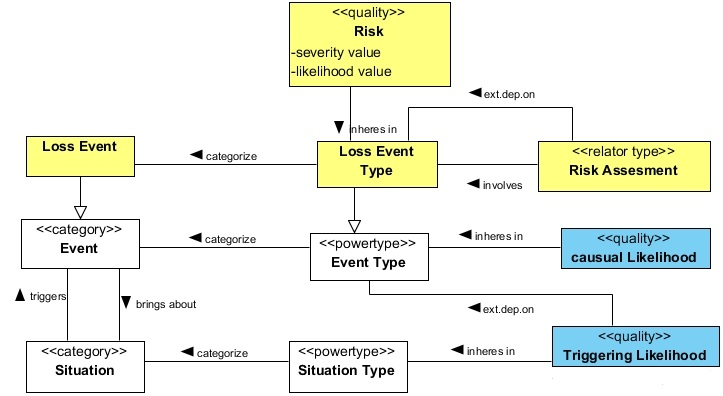
\includegraphics[width=\textwidth]{riskpr.jpg}
\end{center}
\caption{Risk Likelihood in STAMP. Adopted and updated  from~\cite{unknown}ِ}
\label{fig:riskpr}
\end{figure*} 
In Figure~\ref{fig:riskpr}, we represent the likelihood of loss event and risk as a quality in term of UFO type \cite{CARVALHO20173, gagc2015toap}. In \cite{unknown}, they differentiate between a Triggering Likelihood, which inheres in a Situation Type and represents how likely a Situation Type will trigger an Event Type once a situation of this type becomes a fact, and a Causal Likelihood that inheres in an Event Type and represents how likely specific event e will cause another event type to occur. Risk as a quality should indicate two values in safety. First is severity that depends on the type of loss (e.g. if the loss event leads to death then the severity value is high but if it results in only small damages, the severity value is low etc.) and second is probability, combining probabilities of individual failures in event model chain.

 Regarding STAMP \cite{leveson2012engineering}, probabilistic risk assessment (PRA) is not appropriate for systems controlled by software and by humans making cognitively complex decisions. There is no effective way to incorporate management and organizational factors, such as flaws in the safety culture, into PRA despite many well-intentioned efforts to do so. As a result, these critical factors in accidents are often omitted from risk assessment because analysts do not know how to obtain a “ failure ” probability, or alternatively, a number is pulled out of the air for convenience. If we knew enough to measure these types of design flaws, it would be better to fix them than to try to measure them. Another possibility for future progress is usually not considered, and so the conclusion in STAMP is that "Risk and safety may be best understood and communicated in ways other than probabilistic risk analysis"~\cite{leveson2012engineering}.
 
 Nevertheless, STAMP does not reject probability value as a constituent of Risk in general. It only emphasizes that in complex systems this value is untraceable and for the purpose of achieving practical results of the Risk analysis, the value needs to be replaced by other variables, such as mitigation potential~\cite{Leveson2009}. In this paper, however, we aim to propose formalization of the base PRA approach and so adhere to the standard probability inclusion. In future work concerning the overall STAMP ontology, we will address the need for offsetting the issues related to Risk assessment in complex systems, which will be possible by extending the ontologial foundations provided in this work.


\section{STAMP Control Loop Hazard Profile Ontology}
\label{sec:sclhp}
In this section we describe the SCLHP ontology.

\section{Analyzing STAMP Hazard and Risk in term of UFO}
In the previous section, we discussed SHRO in terms of the Common Ontology of Value and Risk \cite{unknown}. In this section, we describe SHRO main concepts in term of UFO and OntoUML.

Fig.~\ref{fig:f2} presents SHRO's conceptual model. In this model, the UFO's concepts are in white, Common Ontology of Value and Risk concepts are in blue and the concepts introduced by SHRO are in yellow. 

Building safer systems requires pouting emphasis on system hazards and eliminating or reducing their occurrence. Therefore, the \term{Occurrence} concept is a safety term that refers to the loss event that is caused by system hazards. \term{Occurrence} is a risk event i.e. a perdurant having endurants (UFO: Object) as its participants regarding UFO. Axiom \ref{ax:a1} holds this notion. In UFO, an event occurs in a certain situation at a certain point in time and transforms it to another situation. In SHRO model we refer to this situation as \term{Resulting Situation}. Examples of some \emph{occurrences} (UFO: Event) that may occur in STAMP model-based safety system: two aircraft collided because of the lack of coordination between the airborne TCAS (collision avoidance) system and the ground air traffic controller, each giving different and conflicting advisories on how to avoid a collision. Another example is an \emph{Accident} where one or several components failed, leading to a system failure. And the last example could be crash accident due to coordination problems in the control of boundary areas \cite{leveson2012engineering}. In these three examples, regrading UFO principles, each them are events that have starting and ending time.

% The \term{Hazard} which is the main concept in our ontology that aims to help in analyzing safety occurrences or accidents.
Hence, in UFO Events existentially depend on the objects that participate in them And an event is manifestation of a disposition of an object, then a risk event occurs due to the dispositions of its participants, which are in STAMP model the \term{Hazards} (i.e., the dispositions). Therefore, we consider \emph{Hazard} as dispositions in SHRO conceptual model. In UFO, dispositions are defined as properties that inhere in particular objects and are only manifested in particular situations on the occurrence of certain triggering events, and that can also fail to be manifested \cite{Guizzardi2014}. When manifested, they are manifested through the occurrence of resulting events and state changes. When dispositions enable undesired events, they are referred to as vulnerabilities or here in our model as hazards (Axiom \ref{ax:a4} holds this notion). For example, the flaws in process creation in a safety system is manifested in system failure. And the inadequate in the control loop controller experience makes him susceptible to do mistakes. 
% \COMMENT{ AL: (The examples in the last two sentences in this paragraph are completely unclear to me. Please revise.)}

Accident causal analysis based on STAMP starts with identifying the safety constraints that were violated by hazardous states. \term{UFO-C} \cite{Guizzardi2010a} defines requirement as a Goal, i.e. the propositional content of an Intention that inheres in an Agent. However, there is no obvious definition of constraints in UFO. STAMP defines safety constraints as part of system requirements that must be enforced to prevent hazard's occurrences \cite{leveson2012engineering}. Axiom \ref{ax:a3} explains this argument that having a hazard's occurrence means that, a safety constrain is violated by this hazard. Therefore, in our model \term{Constraint} is a specialization of \term{Requirement} which is \term{UFO-C: Goal}. For example, 
the safety-related design constraint might be, obstructions in the path of a closing door must be detected and the door closing motion reversed. And the system safety requirement or constraint is that the temperature in the reactor must always remain below a particular level~\cite{leveson2012engineering}.
\paragraph{The previous analyzing of SHRO ontology in term of UFO fall into the the same alignment between SHRO and risk value ontology, which lead to verify the SHRO in term of risk value ontology}

% Thus, HRO consists of the common hazards and risk domain concepts, such as objects (e.g.,
% aircraft, crew, aerodrome) and events (e.g. 
% ight, accident) [10]. Figure 3 depicts
% basic concepts in Aviation Safety Ontology that are represented in UFO.
% HRO aims to capture the complex nature of Hazards and the resulted risks.
% create competency questions that the ontology aims to answer.
\section{Validation}
For validation, we consider the \sabio{} guidelines methodology for ontology verification and validation~\cite{DeAlmeidaFalbo2014}.
\subsection{SHRO Verification}
To verify our ontology, we answer the constructed competency questions \term{(CQs)} by domain expert that he used to find the best answers directly from the STAMP theory~\cite{leveson2012engineering}, then we mapped these answers to the ontological axioms defined before, and check the conceptualization of our ontology by highlighting its concepts and relations in the answers. We highlight only SHRO concepts, we don't highlight STAMP or UFO ontology terms. The results are shown in table~\ref{tab:my1}.

\begin{table*}\label{tab:my1}\caption{Ontology verification}
\begin{tabular}{|p{5cm}|p{8cm}|l|} 
    \hline
CQS& Answers with highlighting ontology relations and concepts & Axioms \\
\hline
$CQ_1$: Where can be identified responsibility for specific risks? &  The responsibility for implementing each \textbf{requirement} needs to be assigned to the components of the control structure, along with requisite authority and accountability, as in any management system; \textbf{controls} must be designed to ensure that the responsibilities can be carried out; and \textbf{feedback loops} created to assist the \textbf{controller} in maintaining accurate process models. & -\\
$CQ_2$: Which objects participate in a specific occurrence? & \textbf{Objects} \textbf{participating} in a specific \textbf{occurrence} are given by the safety control structure in place to control the \textbf{hazard} and enforce the safety \textbf{constraints}. This structure includes the roles and responsibilities of each component in the structure as well as the \textbf{controls} provided or created to execute their responsibilities and the relevant feedback provided to
them to help them do this. & A1 \\ 
$CQ_3:$ How does risk accumulate concerning specific hazard? & The basic STAMP concept is that most major \textbf{accidents} does not result simply from a unique set of proximal, physical \textbf{events} but from the migration of the organization to a state of heightened \textbf{risk} over time.  &  -\\
$CQ_4:$ Why a specific accident happens?& If there is an \textbf{accident}, one or more of the following \textbf{hazards} must have occurred: (1) the safety \textbf{constraints} were not enforced by the \textbf{controller}, (2) appropriate \textbf{control actions} were provided but not followed. & A3 \\
$CQ_5:$ What are the hazards in the controlled system? & \textbf{Hazards} are system states or set of conditions that, together with a particular set
of worst-case environmental conditions, will lead to an \textbf{accident} or \textbf{loss}.  & A4 \\ 
$CQ_6:$ What is the STAMP failure classification? & Classification of \textbf{accident} causal \textbf{factors} starts by examining each of the basic components of a \textbf{control loop} and determining how their improper operation may \textbf{contribute to} the general types of \textbf{inadequate control} or \textbf{hazard}. The causal \textbf{factors} in \textbf{accidents} can be divided into three general categories: (1) the \textbf{controller} operation, (2) the behavior of \textbf{actuators}
and controlled processes, and (3) communication and coordination among
\textbf{controllers} and decision makers.  & - \\
$CQ_7:$ Where is the potential for inadequate control actions (possible control flaws)? & \textbf{Inadequate control} includes cases where (a) the \textbf{control actions} necessary to enforce the associated safety \textbf{constraint} at each level of the socio-technical control structure for the system were not provided, (b) the necessary control actions were provided but at the wrong time (too early or too late) or stopped too soon, (c) unsafe control actions were provided that caused a \textbf{violation} of the safety \textbf{constraints}. & A3 \\
$CQ_8:$ What is an accident? &  \textbf{Accident} is an undesired and \textbf{unwanted event} or an \textbf{occurrence} that results in a \textbf{loss} of some \textbf{severity} (including \textbf{loss} of human life or injury, property damage, environmental pollution, and so on). Losses result from different \textbf{hazards} such component failures, disturbances external to the system, interactions among system components, and behavior of individual system components that lead to hazardous system states. & A4 \\
% $CQ_9:$ Which hazards violated? the constraints &  & \\
\hline
\end{tabular}
\end{table*}

\subsection{SHRO Validation }
\label{Validation}
To validate the ontology, we instantiated some of the defined competency questions using the industry example from section~\ref{sec:example} regarding the helicopter shot down accident. Then, we tested these instances in our ontology, we mapped between expected Outputs and SHRO matching concepts if exist. The selection of instances is done by the domain expert. Table~\ref{tab:my2} shows the instances. In addition, we create a conceptual model for this example, in order to analyze the accident based on our ontology. It is depicted in Figure~\ref{fig:f3}. The example's concepts are in orange color.
 \begin{figure*}
\begin{center}
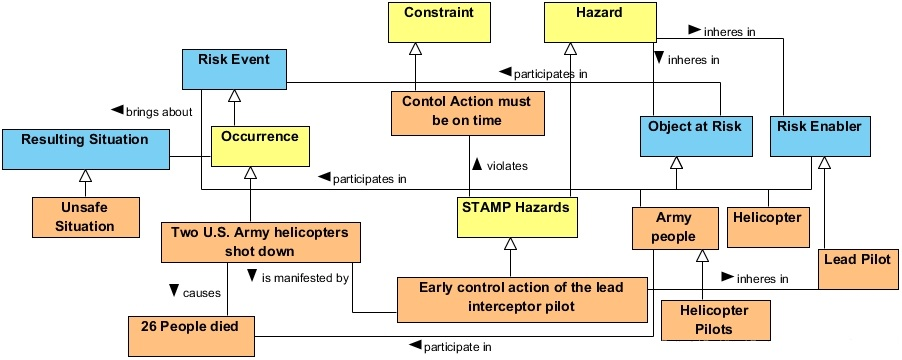
\includegraphics[width=\textwidth]{hexample.jpg}
\end{center}
\caption{Conceptual model of U.S. helicopters shot down accident}
\label{fig:f3}
\end{figure*}

\begin{table*}\label{tab:my2}\caption{Ontology validation}
\begin{tabular}{|p{6cm}|l|p{6.5cm}|} 
\hline
CQS Instances& \textbf{Input} & \textbf{Expected Output with SHRO matching concept if exists} \\
\hline
$CQI_1$: Who was responsible for visual identification of unidentified flying objects?(instantiated from CQ7)  &visual identification event & The lead pilot and his wingman \emph{(Risk Enabler)} \\
$CQI_2$:  Which objects participated in the event of the helicopters shot down? (instantiated from CQ8) &  helicopters shot down & Two F-15 fighter aircraft (interceptors) and two UH-60 helicopters \emph{(Object at Risk)} \\
$CQI_3:$  How did the risk accumulate since the visual contact between the fighter aircraft and the helicopters? (instantiated from CQ3) & helicopters shot down &  After the visual contact, the lead fighter pilot conducted visual identification pass and requested confirmation of identification from his wingman. This was received in rather ambiguous way (nor confirming visual contact with enemy helicopters), what was followed by instruction to disarm missiles and the shot down \emph{(Event's Parts, causes)}  \\ 
$CQI_4:$ What are the factors of this accident? (instantiated from CQ4)& helicopters shot down & Many inadequacies have been identified in the safety control structure (violated safety constraints, inadequate control actions etc.) at the time of the accident. All the control issues either directly caused or contributed to the accident \emph{(Hazards)}.  \\
% $CQI_5:$ What were the hazards pertaining potential attack from the fighter aircraft? &  &  \\
% $CQI_6:$ How can be the actions of the leading fighter pilot be classified?&  & \\
% $CQI_8:$ What kind of potential inadequate control actions existed for the leading fighter pilot? &  & \\
% $CQI_8:$&  & \\
% $CQI_9:$ &  & \\
\hline
\end{tabular}
\end{table*}

% Dispositions Models.

% \subsection{Experts judgments}
% \subsection{Benchmark of Queries: Competency Question Instantiating }
\section{Related Work}
From the conceptual model perspective, we are not the first to analyze hazard and risk events. The Common Ontology of Value and Risk that we have discussed in detail in Section~\ref{sec:back:onto:risk} was used as the base for this work. It formally characterizes the process of ascribing risk as a particular case of the process of ascribing value \cite{unknown}. In \cite{6658262}, a well-founded ontology is provided for resources and capabilities modeling in enterprise architecture for ArchiMate. Modeling Enterprise Risk Management and Security with the ArchiMate Language paper identifies the Enterprise Risk Management (ERM) concepts, tests many standards and frameworks for ERM and security deployment, gathers a set of accepted risk by analyzing a representative sample of ERM, analyzes their semantics and describes the capabilities of the ArchiMate 2.1 \cite{d2d92390811345be868098a06f243a96}. In \cite{8089840}, the authors analyse the Risk and Security Overlay also of the ArchiMate language. Goal-Risk approach \cite{Asnar:2011:GRA:1999080.1999082} is another related work which represents a goal-oriented approach for analyzing risks in term of requirements. In \cite{d2d92390811345be868098a06f243a96}, enterprise architecture of risks by Archimate models is analyzed. In addition, in our previous work we proposed an aviation safety ontology that defines the basic concepts from the aviation industry and describes Ramp Error Decision Aid (REDA) Contributing Factors that cause some specific accidents \cite{Kostov2017b}.

\section{Conclusion}
In this paper, we have discussed the ontological foundation of hazard and risk regarding the System-Theoretic Accident Model and Processes (STAMP) in aviation safety domain as a use case. We aligned main STAMP concepts with respect to risk value ontology formalized in OntoUML.
As a result, we proposed STAMP hazard risk ontology (SHRO) which its implementation could help with creating semantic analyses of safety systems accidents and hazards. Moreover, we implemented SHRO in formal ontological language (OWL) which allows creating SPARQL Queries for testing our ontology by instantiating the competency questions \term{(CQs)}.  

\COMMENT{ AL: I think we should consider adding some text to the conclusion. At least the limitations of our work, recommendations and prospects. Beware, that we should also update the abstract to include more of our methodology and results}

% \section*{References}
% References
\bibliographystyle{ios1}           % Style BST file.
\bibliography{bibfile}        % Bibliography file (usually '*.bib')

\end{document}

